\documentclass[10pt, conference, compsocconf]{IEEEtran}
\usepackage[nocompress]{cite}
\usepackage[font=normalsize,labelfont=sf,textfont=sf]{subfig}
\usepackage{graphicx}
\usepackage{arabtex}
%\usepackage[cmex10]{amsmath}

%packages that were not copied from the IEEE template - need to check if it is valid to add them
\usepackage{amssymb}
\usepackage[linesnumbered]{algorithm2e}

\usepackage{etoolbox}
\newtoggle{edit-mode}
\togglefalse{edit-mode}  
%\toggletrue{edit-mode}

\usepackage{amsthm}

\theoremstyle{definition}
\newtheorem{definition}{Definition}[section]

\begin{document}

\title{Fast technique for On-line Arabic Character Classification Using Earth Movers Distance Embedding to Wavelets Domain}

\author{\IEEEauthorblockN{George Kour}
\IEEEauthorblockA{Faculty of Engineering\\
Tel-Aviv University\\
Tel-Aviv Jaffa, Israel\\
Email: georgeko@post.tau.ac.il}
\and
\IEEEauthorblockN{Raid Saabne}
\IEEEauthorblockA{Department of Computer Science\\
Tel Aviv-Yaffo Academic Collage, Israel\\
Triangle R\&D Center, Kafr Qara, Israel\\
Email: saabni@cs.bgu.ac.il}
}

\maketitle

\begin{abstract}

\end{abstract}

\begin{IEEEkeywords}

Arabic script segmentation; handwriting recognition; on-line text segmentation; 
\end{IEEEkeywords}

\section{Introduction}

\begin{enumerate}
\item Concentrate on the idea of embedding the letters into the wavelet domain. The reason for doing so is to achieve a huge speedup in the recognition without giving up accuracy.
\item Maybe it brings back the k-NN 
\item talk about the segmentation paper, for which this classification system was used.
\item How to test the accuracy of the scoring.
\end{enumerate}

The set of limitations
\begin{enumerate}
\item No additional strokes are taken into considerations.
\item letters written in the same stroke.
\end{enumerate}

This study investigates classification of On-line Arabic characters using EMD Approximation techniques.


\iftoggle{edit-mode}{\hspace{0pt}\marginpar{General motivation and importance}}{}

\iftoggle{edit-mode}{\hspace{0pt}\marginpar{On-line vs. Off-line HWR}}{}

\iftoggle{edit-mode}{\hspace{0pt}\marginpar{Holistic vs. Analytic approach}}{}

\iftoggle{edit-mode}{\hspace{0pt}\marginpar{The gap}}{}

\iftoggle{edit-mode}{\hspace{0pt}\marginpar{Relate to segmentation paper}}{}
This work describes the classifier used to segment on-line handwritten script used the  work done by the authors in \ref{segmentationPaper}.
The real-time nature of the segmentation technique described in \ref{segmentationPaper} strictly requires the classifier to be extremely fast.
The goal of the system is to perform strokes segmentation and letters recognition on-line, i.e., while the stroke is being written thus delays.
The compliance with the high performance demand was made possible by using a state-of-the-art method for fast computation of the approximate $k$-NN which will be described in this paper.

\section{Related Work}
\label{sec:related_work}

\begin{itemize}
\item Raid's paper on EMD embedding
\item papers cited by Raid's paper for letters classification.
\end{itemize}

\section{Our Approach}
\label{sec:approach}
In the presented work, we address the problem of classifying individual Arabic letters.
The unique thing about this classifier is it's speed, which is a critical aspect on real-time On-line script recognition \ref{myPaper}.
The classifier is composed of five stages which includes preprocessing, feature extraction, embedding into the wavelet domain and classification usng $k$-NN classifier.
The classifier is trained and tested using letters extracted from the ADAB database. 
Using a public and not a self collected samples gives our results a further firmness.
The classifier in the work receives a sequence of points representing the letter trajectory and a letter position, and outputs a list of sample candidates and their scoring which indicates the similarity measure between the sequence and the candidate.
The classifier contains four databases, one for each letter position (Ini, Mid, Fin and Iso). 
The partitioning of the samples to four database, clearly, improve the classification power and the accuracy of the classification and scoring.
In Figure \ref{fig:letters_classifier_learning_flow} we give a high level flow visualization of our letters classifier.

A stroke $S$ is represented by a sequence of points on the 2-dimensional space, $p_{i}=(x,y)$ 
\begin{equation}
S=\{p_{i}\}_{i=1}^{n}
\end{equation}
Let $KP$ (Key Points) be zero based ordered set containing the CPs found in the previous sub-stage and that also include the first and the last point of the stroke $S$. Assuming $L$ CPs were found in the stroke $S$, $KP$'s definition is as follows:
%\begin{equation}
%KP_{i} =\begin{cases}    1		, & \mbox{if } i=0 \\
%							   CP_{i}	, & \mbox{if } 1\leq i \leq L \\
%							   n    , & \mbox{if } i=L+1 
%			\end{cases}				
%\end{equation}
A sub-stroke $S_{i}^{j}$ is a sub-sequence of the stroke $S$ that starts at $KP_{i}$ and ends at $KP_{j}$, formally:
\begin{equation}
S_{i}^{j}=(p_{k})_{k=KP_{i}}^{KP_{j}}; i<j
\end{equation}

\begin{figure}
\centering
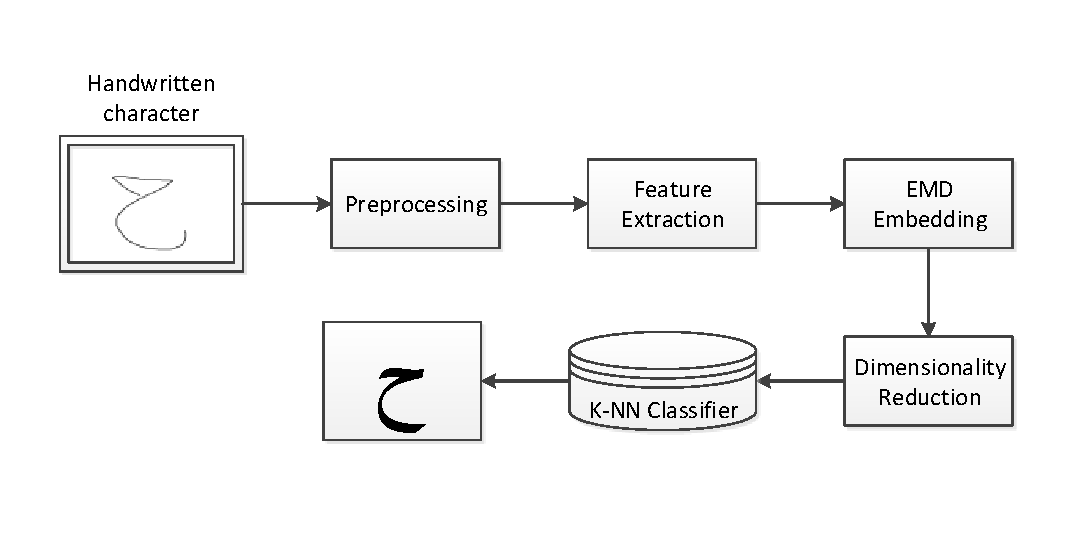
\includegraphics[width=1\columnwidth]{./figures/letters_classifier_learning_flow}       
\caption{High level diagram of the classifier learning flow for a letter position.}
\label{fig:letters_classifier_learning_flow}
\end{figure}

\subsection{Preprocessing}
Digitizers tend to generate a jagged and non-uniform sampling of the trajectory scribed on their surface.
Such devices, normally, sample the input in constant time intervals, thus, slow pen motion regions are over-sampled and fast motion regions are under-sampled.
Further imperfections are caused by hand vibrations resulting from hesitant writing \cite{huang2009preprocessing}.
This lack of uniformity in the data, if not deliberately used by the classification system, should be reduced as much as possible as it could negatively influence the classification system performance.
In order to overcome the flaws mentioned, preprocessing operations are usually needed to impose certain uniform structure on the data, to comply with the input structure required for the proper operation of the subsequent parts of the system \cite{al2011online}. In the current work, preprocessing consists of three methods: \emph{normalization}, \emph{noise elimination} and then \emph{re-sampling}.

\subsubsection{Normalization}
Size normalization is performed to achieve a uniform size of the bounding box surrounding the pattern. 
It was applied on each stroke so that it will fit into a $[0,1]\times[0,1]$ bounding box without affecting the original aspect ratio. 
This stage includes an additional step of translating the sequence so that the sequence's center of gravity is located in the origin point, i.e., at $[0,0]$.
%
%Given the stroke sequence $S=\{p_i\}_{i=1}^{n}=\{(x_i,y_i)\}_{i=1}^{n}$, the normalized sequence $\bar{S}=\{\bar p_i \}_{i=1}^{n}=\{(\bar x_i,\bar y_i)\}_{i=1}^{n}$ is calculated by: 
%\begin{equation}
%{\bar x_i} = {{\left( {{x_i} - {\mu _x}} \right)} \over W},{\bar y_i} = {{\left( {{y_i} - {\mu _y}} \right)} \over W}
%\end{equation}
%where $W = \max (d_x,d_y)$, $d_x$ and $d_y$ are the width and hight of the pattern, respectively, and $\mu$ is the center of gravity of the patter, i.e., 
%\begin{equation}
%\mu  = \left( {{\mu _x},{\mu _y}} \right) = \left( {{1 \over N}\sum\limits_{i = 1}^N {{x_i}} ,{1 \over N}\sum\limits_{i = 1}^N {{y_i}} } \right)
%\end{equation}

\subsubsection{Noise Elimination}

The input obtained by the digitizer usually contains a large amount of noise irrelevant for pattern classification. 
This noise consists mainly of redundant successive points duplication and inadequacies caused by hand vibrations. 
The \emph{Douglas-Peucker Polyline Simplification algorithm} described in \cite{douglas1973algorithms}, also known as the \emph{Iterative Endpoint Fit} algorithm, was used for eliminating such deficiencies in the data. 

The algorithm reduces the number of vertices in a piecewise linear curve, given a preset tolerance parameter $\varepsilon$, which defines the maximum 'dissimilarity' between the original and the reduced curve.
It outputs a simplified curve, that consists of a subset of the points that defined the original curve.
In this work the tolerance parameter $\varepsilon$ was empirically set to ${1 \over 75}$.

\subsubsection{Re-sampling}
The Noise Elimination process produces a highly angular, and non-uniform distribution of points along the stroke trajectory.
Naturally, there are less points in straight areas and a higher density of points in the curved areas stroke. 
This stage, using splines interpolation method, aims to produce an equidistant smoothed data sequence, given a re-sampling target number of points $R$, which was set to 40. 
Given a stroke $S=\{(x_i,y_i)\}_{i=1}^{n}$, let $f_{x}(d)$ and $f_{y}(d)$ be the quadratic piecewise interpolations function of $\{x_i\}_{i=1}^{n}$ and $\{y_i\}_{i=1}^{n}$, respectively. 
$f_{x}(d)$ and $f_{y}(d)$ are functions of the coordinate value with respect to the arc-length distance from the pattern's starting point. 
Let $t_i=i\frac{L}{R}$ for $i=0,...,R$ where L is the arc-length of the pattern.
The re-sampled sequence is given as follows:
\begin{equation}
\widehat{S}=\{(f_x(t_i),f_y(t_i))\}_{i=1}^{R}
\end{equation}

Figure \ref{fig:before_after_preprocessing} demonstrate the re-sampling steps.

\begin{figure}
	\centering
        \subfloat[]{
            \label{fig:preprocessing_orig}
            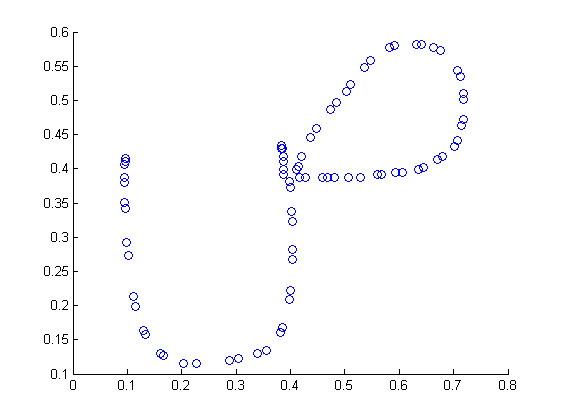
\includegraphics[width=0.4\columnwidth]{./figures/preprocessing_orig}
        }
        \subfloat[]{
           \label{fig:preprocessing_norm}
           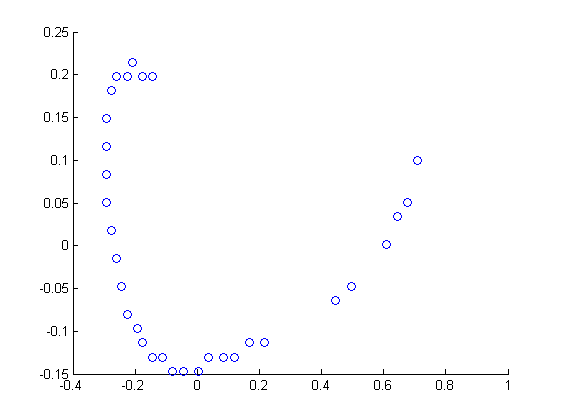
\includegraphics[width=0.4\columnwidth]{./figures/preprocessing_norm}
        }  \\
        \subfloat[]{
            \label{fig:preprocessing_simpl}
            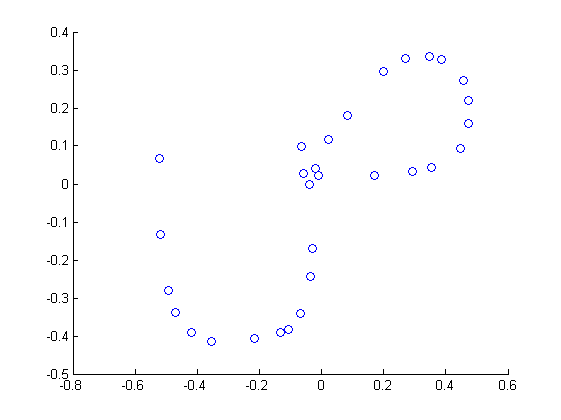
\includegraphics[width=0.4\columnwidth]{./figures/preprocessing_simpl}
        }
        \subfloat[]{
           \label{fig:preprocessing_resamp}
           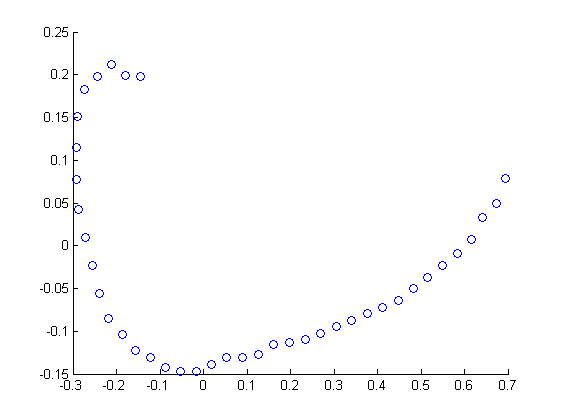
\includegraphics[width=0.4\columnwidth]{./figures/preprocessing_resamp}
        }       
    \caption{A sample of the letter \RL{b} before preprocessing (a); after normalization (b); after noise elimination (c) and after re-sampling (d).}
   \label{fig:before_after_preprocessing}
\end{figure}


\subsection{Feature Extraction}

\iftoggle{edit-mode}{\hspace{0pt}\marginpar{Selected Descriptors}}{}
In this work we have chosen to work with two shape descriptors, the Shape context descriptor and the MAD feature. 

\iftoggle{edit-mode}{\hspace{0pt}\marginpar{Shape Context}}{}
Belongie and Malik have presented a point matching approach named \emph{Shape Context} \cite{belongie2002shape}. 
The Shape context is a shape matching approach that intended to be a way of describing shapes that allows for measuring shape similarity and the recovering of point correspondences. 
This approach is based on the following descriptor: Pick $n$ points on the shape's contour, for each point ${p_i}$ on the shape, consider the $n - 1$ other points and calculate the coarse histogram of the relative coordinates. Equation \ref{eq:sc_bins} is defined to be the shape context of point ${p_i}$.
\begin{equation}
{h_i}(k) = \# \{q \ne p_i:(q - p_i) \in bin(k) \}
\label{eq:sc_bins}
\end{equation}
The bins are normally taken to be uniform log-polar space making the descriptor more sensitive to positions of nearby sample points than to those of points farther away. 
This distribution over relative positions is robust and compact, yet highly discriminative descriptor. 
The basic Idea of the Shape Context Descriptor is illustrated in Figure \ref{fig:shape_context_demo}. 
Shape Context can be calculated in $O(N^3)$ time using the Hungarian method.

\begin{figure}
\centering
\label{fig:shape_context_online}
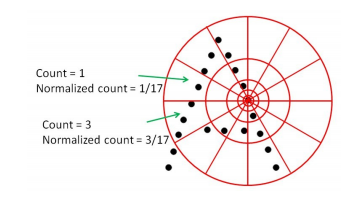
\includegraphics[width=0.3\columnwidth]{./figures/shape_context_online}
\caption{Diagram of the log-polar bins used to compute the shape context.}
\label{fig:shape_context_demo}
\end{figure}

The other feature set is the \emph{Multi Angular Descriptor} (MAD) that was proposed by Saabni in \cite{saabni2013multi}. 
It captures the angular view to multi resolution rings in different heights. 
The shape is treated as a two dimensional set of points and the different rings are upper view points from rings around the shape centroid with different sizes and heights. 
To enables scale and translation invariance, the sizes and heights of these rings are calculated using the diameter and centroid of the shape.
Formally, let $S$ be a shape and Let $C$ and $D$ be the centroid and the diameter of the shape respectively. 
Let $P = \{p_i\}_{i = 1}^l$ a set of $l$ point taken uniformly from the extracted contour of $S$. Given a view point $V_j$ from a given ring with height $h$ over the shape, the angle, obtained by connecting the point ${p_i} \in P$ with each point and the plain of the shape is a rich description of the shape from this view point. Let $R$ be a ring with the radius $r$ and the center $C$ positioned above the shape $S$ with the height $h$. Let $V = \{V_i\}_{i = 1}^n$ be a set of $n$ viewpoints lying uniformly on the ring $R$ and $\alpha(V_{ij})$ to be the angle between the segment $\overline {{V_i}{p_j}}$ and the plain contains the shape $S$. The vector $Ve{c_i} = \left\{ {\alpha \left( {{V_{ij}}} \right)} \right\}_{j = 1}^l$ can be seen as watching the shape $S$ from one upper view point $V_i$. Illustration can be seen in Figure \ref{fig:mad_demo}.
Figure \ref{fig:mad_demo} provides a visual demonstration of the MAD feature where An example of three line segments drawn from the same viewpoint $V_i$, generating the three angles $Vec_{ij}$ with the plane of the shape. When the parameter $j$ goes over all contour points we get the vector $Vec_i$ describing the shape from the view point $V_i$ with the parameter $i$ goes over all viewpoints.

\begin{figure}
\centering
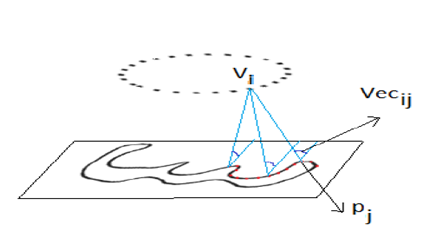
\includegraphics[width=0.5\columnwidth]{./figures/mad_demo}       
\caption{Multi Angular Descriptor}
\label{fig:mad_demo}
\end{figure}

\subsection{Metric Embedding}
\subsubsection{The Earth Mover's Distance}
Histogram based descriptors, such as the Shape Context, are in many cases compared using a bin-wise dissimilarity techniques such as the Minkowski distance or the $\chi^2$ statistic.
Bin-wise dissimilarity measures can be computed very fast due to the fact that they measure dissimilarities between the content of corresponding bins of the two histograms and discard information across bins. 
Thus, they usually fail to consider local and global variations. 
These variations, which would be perceived as minor by a human, may result in a large dissimilarity values between two histograms. 

Generally speaking, the distance between two histograms can be viewed as a special case of the well-known \emph{transportation problem}, a.k.a the Monge-Kantorovich problem \cite{rachev1985monge}.
The \emph{Earth Mover's Distance} (EMD), introduced by Rubner et al. in \cite{rubner2000earth}, is a solution to the transportation problem which can be used as a measure of the dissimilarity between histograms. 
EMD was experimentally verified to capture well the perceptual notion of a difference between images and is commonly used in content-based image retrieval to compute distances between the color histograms of two digital images \cite{grauman2004fast}.
EMD was used by Saabne in \cite{saabni2013efficient} to measure similarity between shapes for recognizing and searching Arabic words. 
However, for the best of our knowledge, this is the first use of EMD for on-line handwriting recognition.

The major hurdle in using EMD is its $O\left( {{N^3}\log N} \right)$ computational complexity (for an $N$-bin histogram). The complexity is magnified when the task is to search for similar shapes (nearest neighbors) in a large database. 
In this case, a linear scan of the database would require computing a comparison of superpolynomial complexity for each database member against the query shape \cite{grauman2004fast}. 
Greatly reducing the EMD calculation time can be achieved using approximation technique. 
One Such approximation technique will be discussed later in this paper. 


\subsubsection{Approximating EMD using Embedding}
\label{subsec:approximating_emd_using_embedding}
Several approximation algorithms have been proposed to speedup the computation of EMD. 
Indyk and Thaper \cite{indyk2003fast} proposed a technique for embedding the un-normed EMD metric into the $L_1$ space so that the EMD distance between the two objects is comparable to the Manhattan distance between the two points which represent the embedding of the two objects.
Approximating the EMD distance between the set $A$ and $B$ is then done by calculating the Manhattan distance between the two corresponding embedding vectors, i.e.,
\begin{equation}
EMD_{approx.}=|f_{EMD}(A) - f_{EMD}(B)|
\end{equation}  
The time complexity of the embedding is $O(Nd \log{\Delta})$, where $\Delta$ ...
The distortion of the embedding has an upper bound of $O(\log \Delta)$. 
A detailed proof is provided in \cite{indyk2003fast}.
However, the proved theoretical distortion can only provide a weak practical instrument. 
Nevertheless, experimental validation performed on a dataset of $20,000$ objects showed a $(1+\epsilon)-approximate$ nearest neighbor, with $\epsilon < 20\%$ achieved by the embedding compared to the exact EMD in \cite{indyk2003fast}. Grauman and Darrel \cite{grauman2004fast} have used this embedding for contour matching and experimentally validated the quality of retrieval. 
They have found that the accuracy reduction is less than $10\%$ compared to the exact EMD.

In a subsequent work done by Shirdhonkar and Jacobs \cite{shirdhonkar2008approximate}, the authors proposed a method for approximating the EMD between two low dimensional histograms using the weighted wavelet coefficients of the difference histogram. 
The approximation is done by transforming the histograms into the $L_1$ space so that the distance between the two vectors in the wavelet domain is the EMD approximation. 
They proved the ratio of EMD to wavelet EMD is bounded by constants. 

Shirdhonkar and Jacobs showed that the embedding of the difference histogram approximates the EMD between two histograms. It is done by calculating the $L_1$ norm of the coefficients vector of the embedding as given in Equation \ref{eq:emd_embedding}.
\begin{equation}
d(p)_{wemd}= \sum\limits_{\lambda} 2^{-j(1+n/2)}|p_{\lambda}|
\label{eq:emd_embedding}
\end{equation}
where $p$ is the n-dimensional difference histogram and $p_{\lambda}$ is the wavelet transform coefficients. 
The index $\lambda$ includes both shifts and the scale j.

Intuitively, the wavelet transform splits up the difference histogram according to scale and location where each coefficient represents the solution to the EMD subproblem. 
For a single wavelet, the mass to be moved is proportional to the volume of $|\psi_j(x)|$, i.e., to $2^{-jn/2}$ and the distance to be travelled is proportional to the span of the wavelet, i.e $2^{-j}$. The sum of all distances is an approximation to EMD, as formally defined in Equation \ref{eq:emd_embedding}. 
This can be viewed as similar to the way packages are shipped over large distances. 
The route is broken into several pieces which are large and small distances. 
Packages from nearby places are merged at the end of the short distance route piece to travel together. 
Then another merge is done of packages from the entire country to be shipped together to the destination country. 
The sum of the distances travelled is an approximation to the actual distance. See Figure \ref{fig:emd_wavelet}.

\begin{figure}
\centering
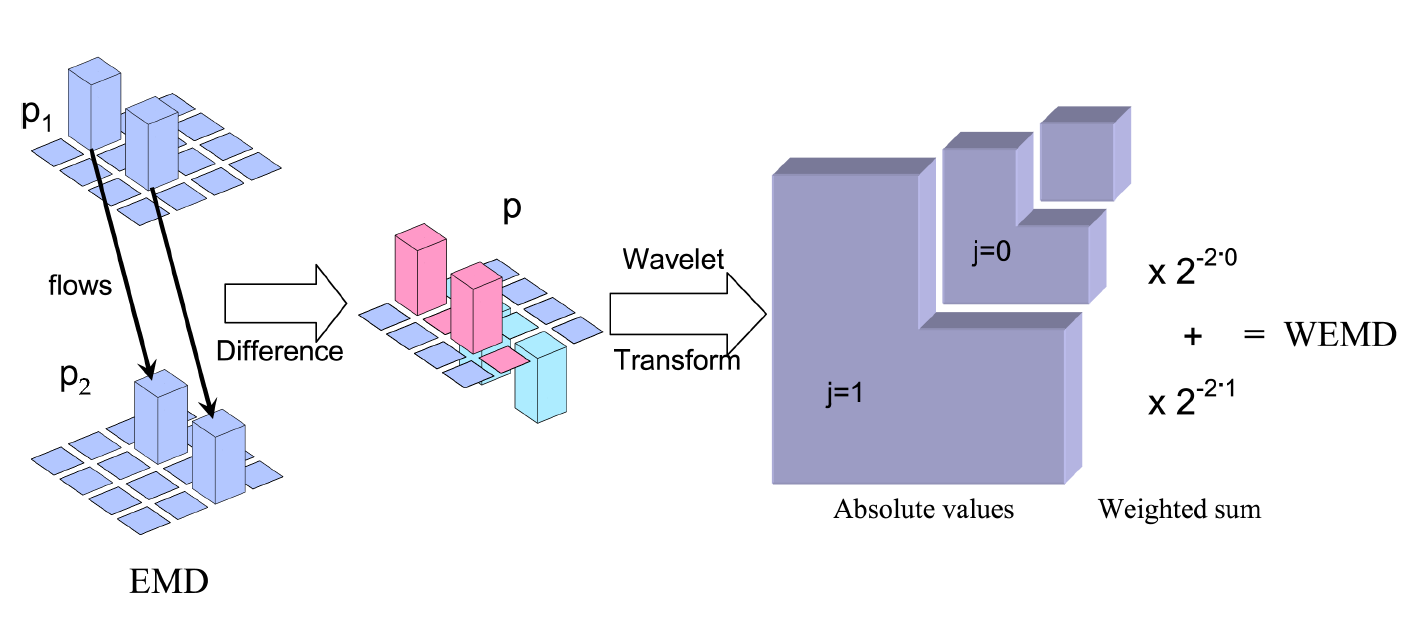
\includegraphics[width=1\columnwidth]{./figures/emd_wavelet}       
\caption{EMD embedding using the wavelet domain \cite{shirdhonkar2008approximate}.}
\label{fig:emd_wavelet} 
\end{figure}

However, in our application, where the histogram descriptors are to be stored rather than the difference histogram, the computation of EMD can be partitioned into two parts. 
First the histograms are converted into the wavelet domain and their coefficients are scaled according to Equation \ref{eq:emd_embedding}. 
Computing the EMD distance, in the next step, is done by calculating the Manhattan distance between the scaled coefficients of the corresponding histograms.

They provided both theoretical and experimental bounds. 
The theoretical approximation is based on Theorem 2 in \cite{shirdhonkar2008approximate}. 
Using a large dataset, they were able to experimentally establish that the proposed approximation follows the true EMD closely empirically and can be alternatively used without any significant difference in performance. 
The wavelet EMD metric can be computed in $O\left( N \right)$ time complexity. 
The authors tested few wavelets and showed that the Coif-lets of order 3 and the Symmetric Daubechies wavelets of order 5 have lowest error rates. 
We followed their results and have chosen to work with the order 3 Coif-lets.

Empirically, the normalized RMS error obtained by using the wavelet embedding was between in 13\% and 20\% compared to the embedding proposed by Indyk and Thaper which achieved 43\% in the same experiment. In addition, the wavelet embedding surpassed the Indyk and Thaper embedding in time performance. Note that the embedding process requires histograms, thus the vectors in the feature space need to be normalized before using this method.

\subsection{Dimensionality Reduction}
\label{subsec:dr}

\emph{Dimensionality Reduction} is a process of reducing the number of variables taken into consideration in the learning and classification of data. 
The undesired properties of high-dimensional data present many mathematical challenges and practical complications \cite{van2009dimensionality}. 
Ideally, the reduced representation should have a dimensionality that corresponds to the intrinsic dimensionality of the data \cite{van2009dimensionality} which is the minimum number of parameters needed to account for the observed properties of the data. 

The need for employing dimensionality reduction in this work emerged from the sparse vectors produces by the EMD embedding of the feature vectors into the wavelet coefficient domain which produced vectors in $R^{3946}$. 
The wish to employ k-d trees, which is very sensitive to high dimensional data, was the main reason for using dimensionality reduction. 
An alternative was to use a $k$-NN data-structure that performs well with high dimensional data such as LSH \cite{gionis1999similarity}. 

In this work we have used a new technique that applies \emph{principle component analysis} (PCA) and \emph{linear discrimination analysis} (LDA) sequentially in order to obtain linearly discriminative information efficiently.
PCA is unsupervised in the sense that the labelling of the data do not effect the determination of the transformation function. 
It produces an orthogonal linear transformation that transforms the data to a new coordinate system such that the greatest variance by any projection of the data comes to lie on the first coordinate (the first principal component), the second greatest variance on the second coordinate, and so on.

The representation content $g$ for the $j^{th}$ eigenvector is the sum of the energy content across all of the eigenvalues $\lambda_k$ from 1 through $j$ :
\begin{equation}
g[j]=\sum_{k=1}^{j}\lambda_k  for  j=1,...,d
\end{equation}
where $d$ denotes the dimensionality of the original data. The \emph{data preservation rate} value (E) is calculates as seen in Equation \ref{eq:dr_energy}. 

\begin{equation}
E[L] = \frac{g[L]}{g[d]}
\label{eq:dr_energy} 
\end{equation} 

The goal is to find the smallest possible value of $L$ that achieves $E[L]$ value which rise above a pre-set threshold $e$, usually larger than 0.9. 
This approach is a well-known dimensionality estimation technique known as the \emph{eigenvalue-based dimensionality estimator}. 

The major drawback of PCA is that it is an unsupervised technique and as such does not use label information of the data
which may cause ...

LDA, a descendant of the original Fisher-LDA that was proposed by Fisher in \cite{fisher1936use}, overcomes this problem. Unlike PCA, LDA is a supervised technique. 
LDA performs dimensionality reduction while preserving as much of the class discriminatory information as possible. 
LDA has three main drawbacks; the first is that it assumes that the data resides in $L_2$; second, LDA assumes that the distribution of the samples in each class is Gaussian which is not necessarily true for our samples; third, it is much slower to calculate compared to PCA.
Even though LDA is preferred in many application, it does not always outperform PCA. 
In order to optimize discrimination performance in a more generative way, a hybrid dimension reduction model combining PCA and LDA is used in this work.

Grauman et al. in \cite{grauman2004fast} used PCA to find a low-dimensional subspace based on a large sample of the shape context histogram. 
PCA yields the set of bases that define a low-dimensional "shape context manifold". 
Only then the approximate EMD embedding is performed. 
However, we have chosen to perform the stages in a different order. 
First, approximate EMD embedding is performed on the feature vectors, and only then, dimensionality reduction procedure is applied to reduce the dimensionality of the sparse embedded vectors since we would still result in a large sparse vectors constructed by the embedding process.

The basic form of PCA is defined over the $L_2$ space. 
However, the data that is embedded to the wavelet domain was proved to approximate EMD in the $L_1$ space. 
Although $L_1$-PCA techniques were examined in the literature \cite{kwak2008principal}, we decided to use the basic form of PCA, given that $L_2$ estimate $L_1$ fairly well.

In the proposed system, we wanted to exploit the strengthens of both PCA and LDA techniques using the dimensionality reduction process which is outlined as follows: The samples are projected to a subspace $S_1$ using PCA and then to subspace $S_2$ using LDA. In the PCA stage, the target dimensionality, i.e., the number of principal components taken into consideration, is the minimal to achieve data preservation rate of 99\%, i.e., $E=0.99$. As mentioned before, the dimensionality of the original vectors was 3946. The reason we adopted such a high rate is that it was enough to secure a major dimensionality reduction. As seen in table \ref{table:dr_dimensions_results}, the dimensionality was reduced by PCA in two orders of magnitude.

\iftoggle{edit-mode}{\hspace{0pt}\marginpar{Implementation: Clustering and LDA}}{}
Applying LDA directly on the resulted data would have achieved poorer results for the reason that almost all letters in the Arabic writing system have several shapes which are commonly used. 
Furthermore, since LDA regards the labeling of the data samples, trying to group different perceptual shapes in a single class would impinge the dimensionality reduction process. 
In order to overcome this obstacle, we have done the following preprocessing steps: each class was was partitioned into four clusters using $L_1$-k-medoids algorithm and received a different class label, and only then LDA was applied.

As aforementioned, the target number of dimensions of the PCA step were determined according to the data preservation rate parameter which was preset to $E=0.99$. 
This can be calculated easily using the eigenvalues of the covariance matrix. 
However, in the LDA step we have adopted a different approach to determine the target number of dimensions. 
\emph{Intrinsic dimensionality estimation} methods are traditional techniques for estimating the intrinsic dimensionality of a data. 
While there are many techniques, many use the same basic concept. They are based on the observation that for a given data point $x_i$, the number of sample points covered by a hypersphere around the data point with radius $r$ grows proportional to $r^d$, where $d$ is the intrinsic dimensionality of the data manifold around that data sample.  
The function that estimates this relation for a given data point $x_i$ is named \emph{local estimator}.
The estimated intrinsic dimensionality $\hat{d}$ of the dataset is then calculated by averaging over the local estimators of the entire sample set \cite{van2007introduction}.

The dimensionality of the data samples is shown in Figure \ref{table:dr_dimensions_results} for every database. The original data set dimensionality is 3946. The PCA column shows dimensionality of the data after applying PCA. The PCA+LDA column shows the dimensionality of the data after applying LDA subsequently after LDA as described.

\begin{table}
\centering
\begin{tabular}{ | c | c | c | c |}
\hline
Letter position & Number of samples & PCA & PCA+LDA\\
\hline                 
  Iso & 1372 & 29 & 7 \\ 
  \hline
  Ini & 1405 & 39 & 9 \\ 
  \hline
  Mid & 1196 & 36 & 8 \\ 
  \hline
  Fin & 1629 & 27 & 7 \\ 
  \hline
\end{tabular}
\caption{Dimensionality Reduction results}
\label{table:dr_dimensions_results} 
\end{table}

\subsection{Fast k-nearest Neighbour approximation}
In order to speedup queries, index structures are usually built over the sample set. 
The main goal of an index method is to enable efficient retrieval and similarity search, either asymptotically or simply in real wall-clock time. 
It aims at solving the problem of searching $k$-NN in a large set of multi-dimensional points by first building a data structure based on the set of reference points. Then, given a query object, it extracts the $k$-NN using this structure.
The time cost involved in building the index is amortized over the series of queries, and is usually ignored when considering search cost \cite{hetland2009basic}.

ANN methods such as k-d trees and Locality Sensitive Hashing (LSH) \cite{gionis1999similarity} have been successfully applied on a variety of fast similarity retrieval problems. 
However, the key assumption in these procedures is that the objects in the dataset lie in a metric space, i.e., the space satisfies the triangle equality, however, this assumption is not valid for many similarity measure techniques, such as EMD.
In the case of k-d tree, it requires the $L_p$ norm for its operation, which is even a more specific demand.
While the worst case scenario complexity is $O(N)$, the expected complexity of a single $k$-NN query using k-d tree is $O(\log N)$.

The embedding of the deature vectors into the $L_1$ space these metric indexing methods can be applied. 
In our work, sub-strokes classification is done by finding sample letters in the training set that are similar to the shape of the sub-stroke.

k-d tree, a special case of binary space partitioning trees, is a data structure for storing a finite set of points from a $k$-dimensional space. 
It was proposed by Bentley in \cite{bentley1975multidimensional}. 
The approximation of the $k$-NN using k-d tree is done by initially finding the leaf node that represents the class that the query point belongs to. 
Although it is probable that the $k$ nearest neighbors are all contained in a single leaf node, it is not necessarily the case. 
Adjacent leafs may be examined by recursively explore the other child nodes and look for near neighbours. 
Precise details of the algorithm can be found in \cite{bentley1975multidimensional}.

\begin{figure}
\centering
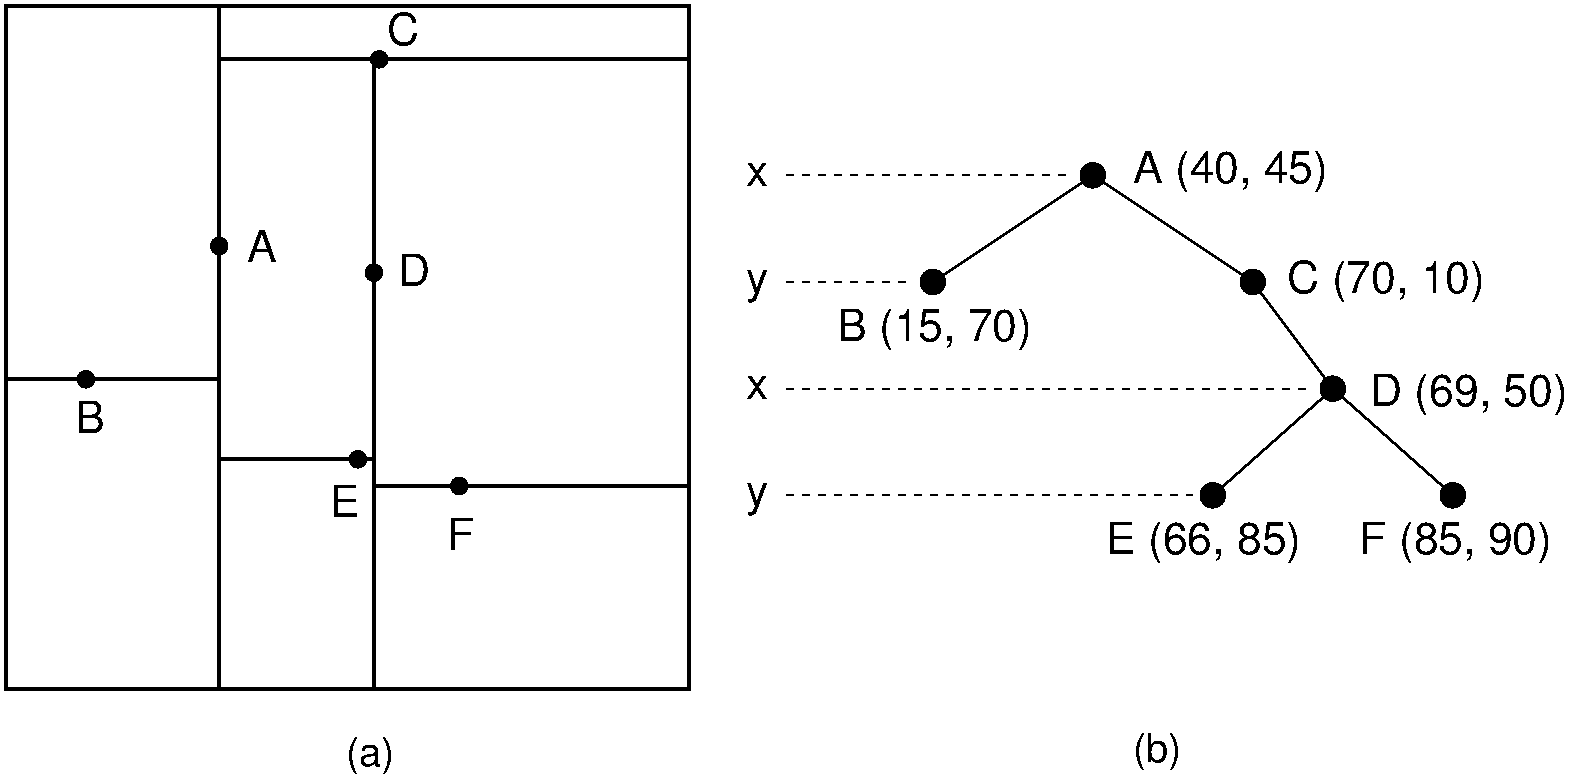
\includegraphics[width=0.7\columnwidth]{./figures/kd_tree}       
\caption{Example of a k-d tree. (a) The k-d tree decomposition  a region containing seven data points. (b) The k-d tree for the region of (a).}
\label{fig:kd_tree}
\end{figure}


\subsection{Candidates Scoring}
For each subsequence, the recognition system returns a set of K potential letters candidates, with their resemblance scoring. 
In the current implementation we consider only the candidate with the best (minimal) scoring, however, any function taking into consideration the scoring returned by the classifier for all the candidate can be used to determine the final scoring of the cell.

Once the set of candidates determined by the closeness found by the k-d tree based on the coefficients vector in the $L_1$ space. The scoring is performed as follows:

The scoring of the candidates is done by averaging the score of the $L_1$ distance between the query object and the candidate in the sample set, and the score of the DTW distance between the feature vector and the 
Let us the denote the feature vector of the query object by $q$ and the feature vector the candidate $i$ by $c_i$.
\begin{equation}
Scoring(c_1)=\frac{EMD_{approx.}(q,c_i)+DTW(q,c_i)}{2} 
\end{equation}

This gives an equal weigth to the DTW and the EMD approximation.
We have found the constraint DTW performs using the unconstrained DTW.
The weights given for each similarity measure technique was determined empirically.


\subsection{Data Collection}
The data is one of the most important part of any supervised learning technique. The data is used for learning, validation and testing. It has a critical effect on the system performance. In this work we have chosen to use the ADAB database. The ADAB database is de-facto a standard in the on-line Arabic handwriting recognition research field. It is freely available and consists of more than 20k Arabic handwritten words scribed by more than 170 different writers. The words are taken from the 937 Tunisian town/village names. It contains the trajectory information and a plot image of the word trajectory. A sample can contain more than a word. In figure \ref{fig:sample_parts} we show the parts of a sample. The ADAB database v.1 is divided to 3 sets. Details about the number of files, words, characters, and writers are given in \cite{el2009icdar}. Our training, validation and testing set both are taken from this database. 
No information relating the strokes to letters or to word-parts is provided, thus, extra work was needed to add this information to the database so that it could be used as letters samples source and also a ground-truth for the segmentation abilities of the system. To provide this additional information, we have created a system that reads the samples from the ADAB database, and employ the skills of a human expert to segment the samples and relate each stroke to the corresponding letter in the WP. The resulted information was saved in an xml file for each word sample. Since additional strokes are not our interest in the segmentation process, the system has automatically filtered out additional strokes. Nevertheless, the human expert had the ability to filter out additional strokes that could not be identified by the system as such. We have manually segmented ~16k samples which consisted about ~40k strokes. 

\section{Results and Analysis}

\emph{TODO: compare with other letter classifiers or digits.}
\emph{TODO: compare the performance of classification without using our approach}

\section{Summary and Future Work}

\section*{Acknowledgment}
The authors would like to thank Professor Dana Ron, from the Tel-Aviv University, for her invaluable help in this research and her insightful comments on this paper. This work has been supported in part by the German Research Foundation under grant no. FI 1494/3-2.

\bibliographystyle{IEEEtran}
\bibliography{IEEEabrv,bibliography}

\end{document}


